\documentclass{article}

\usepackage{fancyhdr}
\usepackage{hyperref}
\usepackage{titlesec}
\usepackage{graphicx}
\usepackage{tikz}

\usetikzlibrary{shapes,arrows}
\newcommand{\comment}[1]{}


\tikzstyle{decision} = [diamond, draw, 
    text width=4.5em, text badly centered, node distance=3cm, inner sep=0pt]
\tikzstyle{line} = [draw, -latex']
\tikzstyle{block} = [rectangle, draw, 
    text width=8em, text centered, rounded corners, minimum height=4em]
\tikzstyle{start} = [rectangle, draw, 
    text width=4.5em, text badly centered, rounded corners, node distance=3cm]
\tikzstyle{io} = [trapezium, trapezium left angle=70, trapezium right angle=110, minimum width=3cm, minimum height=1cm, text centered, draw=black]


\setcounter{secnumdepth}{5}
\setcounter{tocdepth}{4}

\pagestyle{fancy}
\fancyhf{}
\rhead{Path-finding Algorithms and Solving Mazes}
\lhead{Oliver Temple [CN]}
\rfoot{\thepage}
\lfoot{Path-finding Algorithms and Solving Mazes}

\title{Path-finding Algorithms and Solving Mazes}

\author{Oliver Temple}

\begin{document}

\maketitle
\tableofcontents

\section{analysis}
\subsection{Project Description}
Path finding algorithms are essential in many aspects computer science, especially in games and simulations. However, they can be complex things that are hard to visualize, especially when being taught about them. Path finding algorithm visualizers do exist, however, I feel that none of them are perfect, and that they lack features.

Because of this, I am going to make a path finding visualizer that ticks all of the boxes. It will be simple and easy to use, have advanced customization and have the ability to run a path finding algorithms given by the user.

\subsection{Research}
\subsubsection{Overview}
To complete this project, I will need a strong understanding of maze generation and path finding algorithms, how they work and how to model them, knowledge of react and javascript to create a website for the visualization as well as user opinions on what features are needed.
\subsubsection{Research Log}
\paragraph*{Class}
I was introduced to path finding algorithms in one of my lessons, where we learned what they were used for and some examples, as well as how they can be modeled. For example, modelling the maze as a graph with weighted nodes of 1 and 0, for the walls and space respectively. The algorithms we looked at were Dijkstra's and A*. We also looked at Prim's algorithm, recursive backtracking, depth fist search and Kruskal's algorithms for maze generation.

\subsection{Project Background}
\subsubsection{Current Systems}
\paragraph{Example 1}
\href{https://clementmihailescu.github.io/Pathfinding-Visualizer/
}{https://clementmihailescu.github.io/Pathfinding-Visualizer
}
\newline
In this example, mazes can be generated with various algorithms, as well as being drawn by the user. The mazes can also be edited after they have been generated. The available maze generation algorithms are:
\begin{itemize}
    \item Recursive Division
    \item Recursive Division (vertical skew)
    \item Recursive Division (horizontal skew)
    \item Basic Random Maze
    \item Basic Weight Maze
    \item Simple Stair Pattern
\end{itemize}
These mazes can then be solved with a number of different path finding algorithms. The available path finding algorithms are:
\begin{itemize}
    \item Djikstra's Algorithm
    \item A* Search
    \item Greedy Best-first Search
    \item Swarm Algorithm
    \item Convergent Swarm Algorithm
    \item Bidirectional Swarm Algorithm
    \item Breadth-first Search
    \item Depth-first Search
\end{itemize}
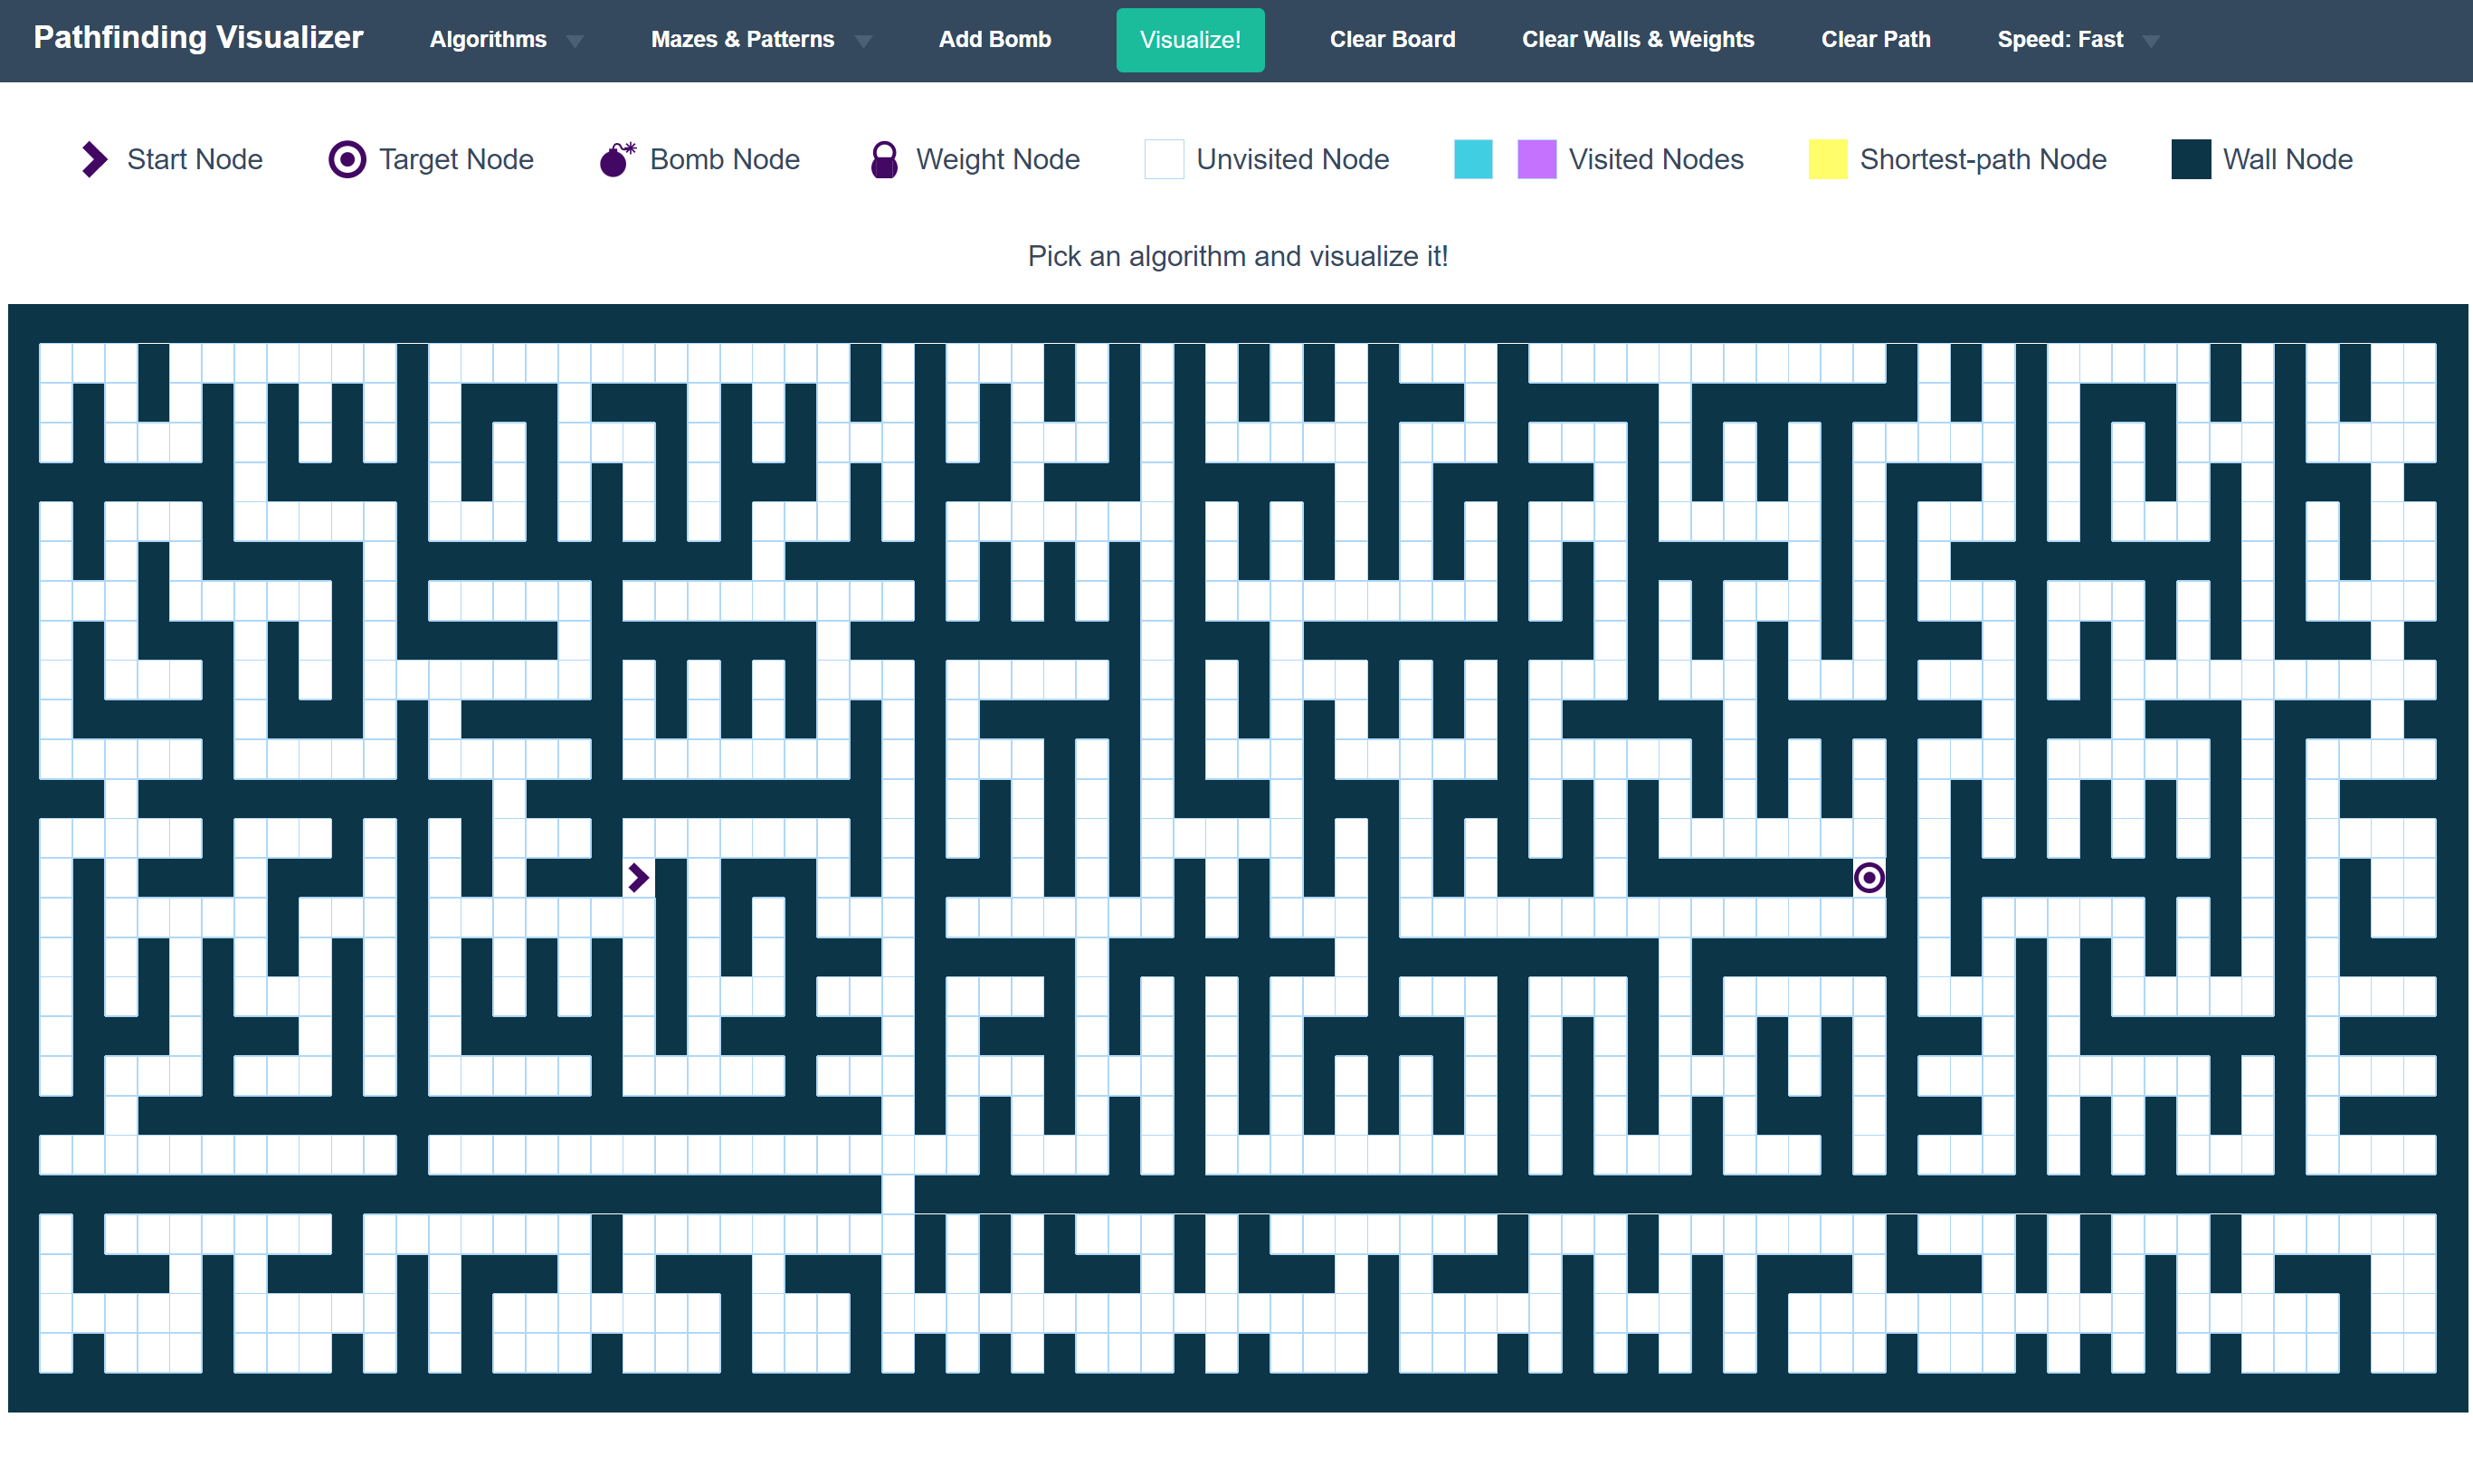
\includegraphics[width=\linewidth]{assets/Existing Solutions/example 1.PNG}
\subparagraph*{pros}
\begin{itemize}
    \item Many different algorithms to choose from.
    \item Start and end nodes can be moved.
    \item Maze can be altered.
    \item If nodes are moved after visualization has run, then the visualization will update.
    \item "Bomb" node, adds a via point that the path must go through.
\end{itemize}
\subparagraph*{cons}
\begin{itemize}
    \item The visualization is too slow.
    \item If maze is altered by user after visualization has run, then the visualization will not update.
\end{itemize}


\paragraph{Example 2}
\href{https://qiao.github.io/PathFinding.js/visual/
}{https://qiao.github.io/PathFinding.js/visual/
}
\newline
In this example, mazes have to be drawn by the user. The maze can then be solved with a number of different algorithms, however, these algorithms have more choice. For example, in the A* option, you can change the heuristic that is used. The available algorithms are:
\begin{itemize}
    \item A*
    \item IDA*
    \item Breadth-First-Search
    \item Best-First-Search
    \item Dijkstra
    \item Jump Point Search
    \item Orthogonal Jump Point Search
    \item Trace
\end{itemize}
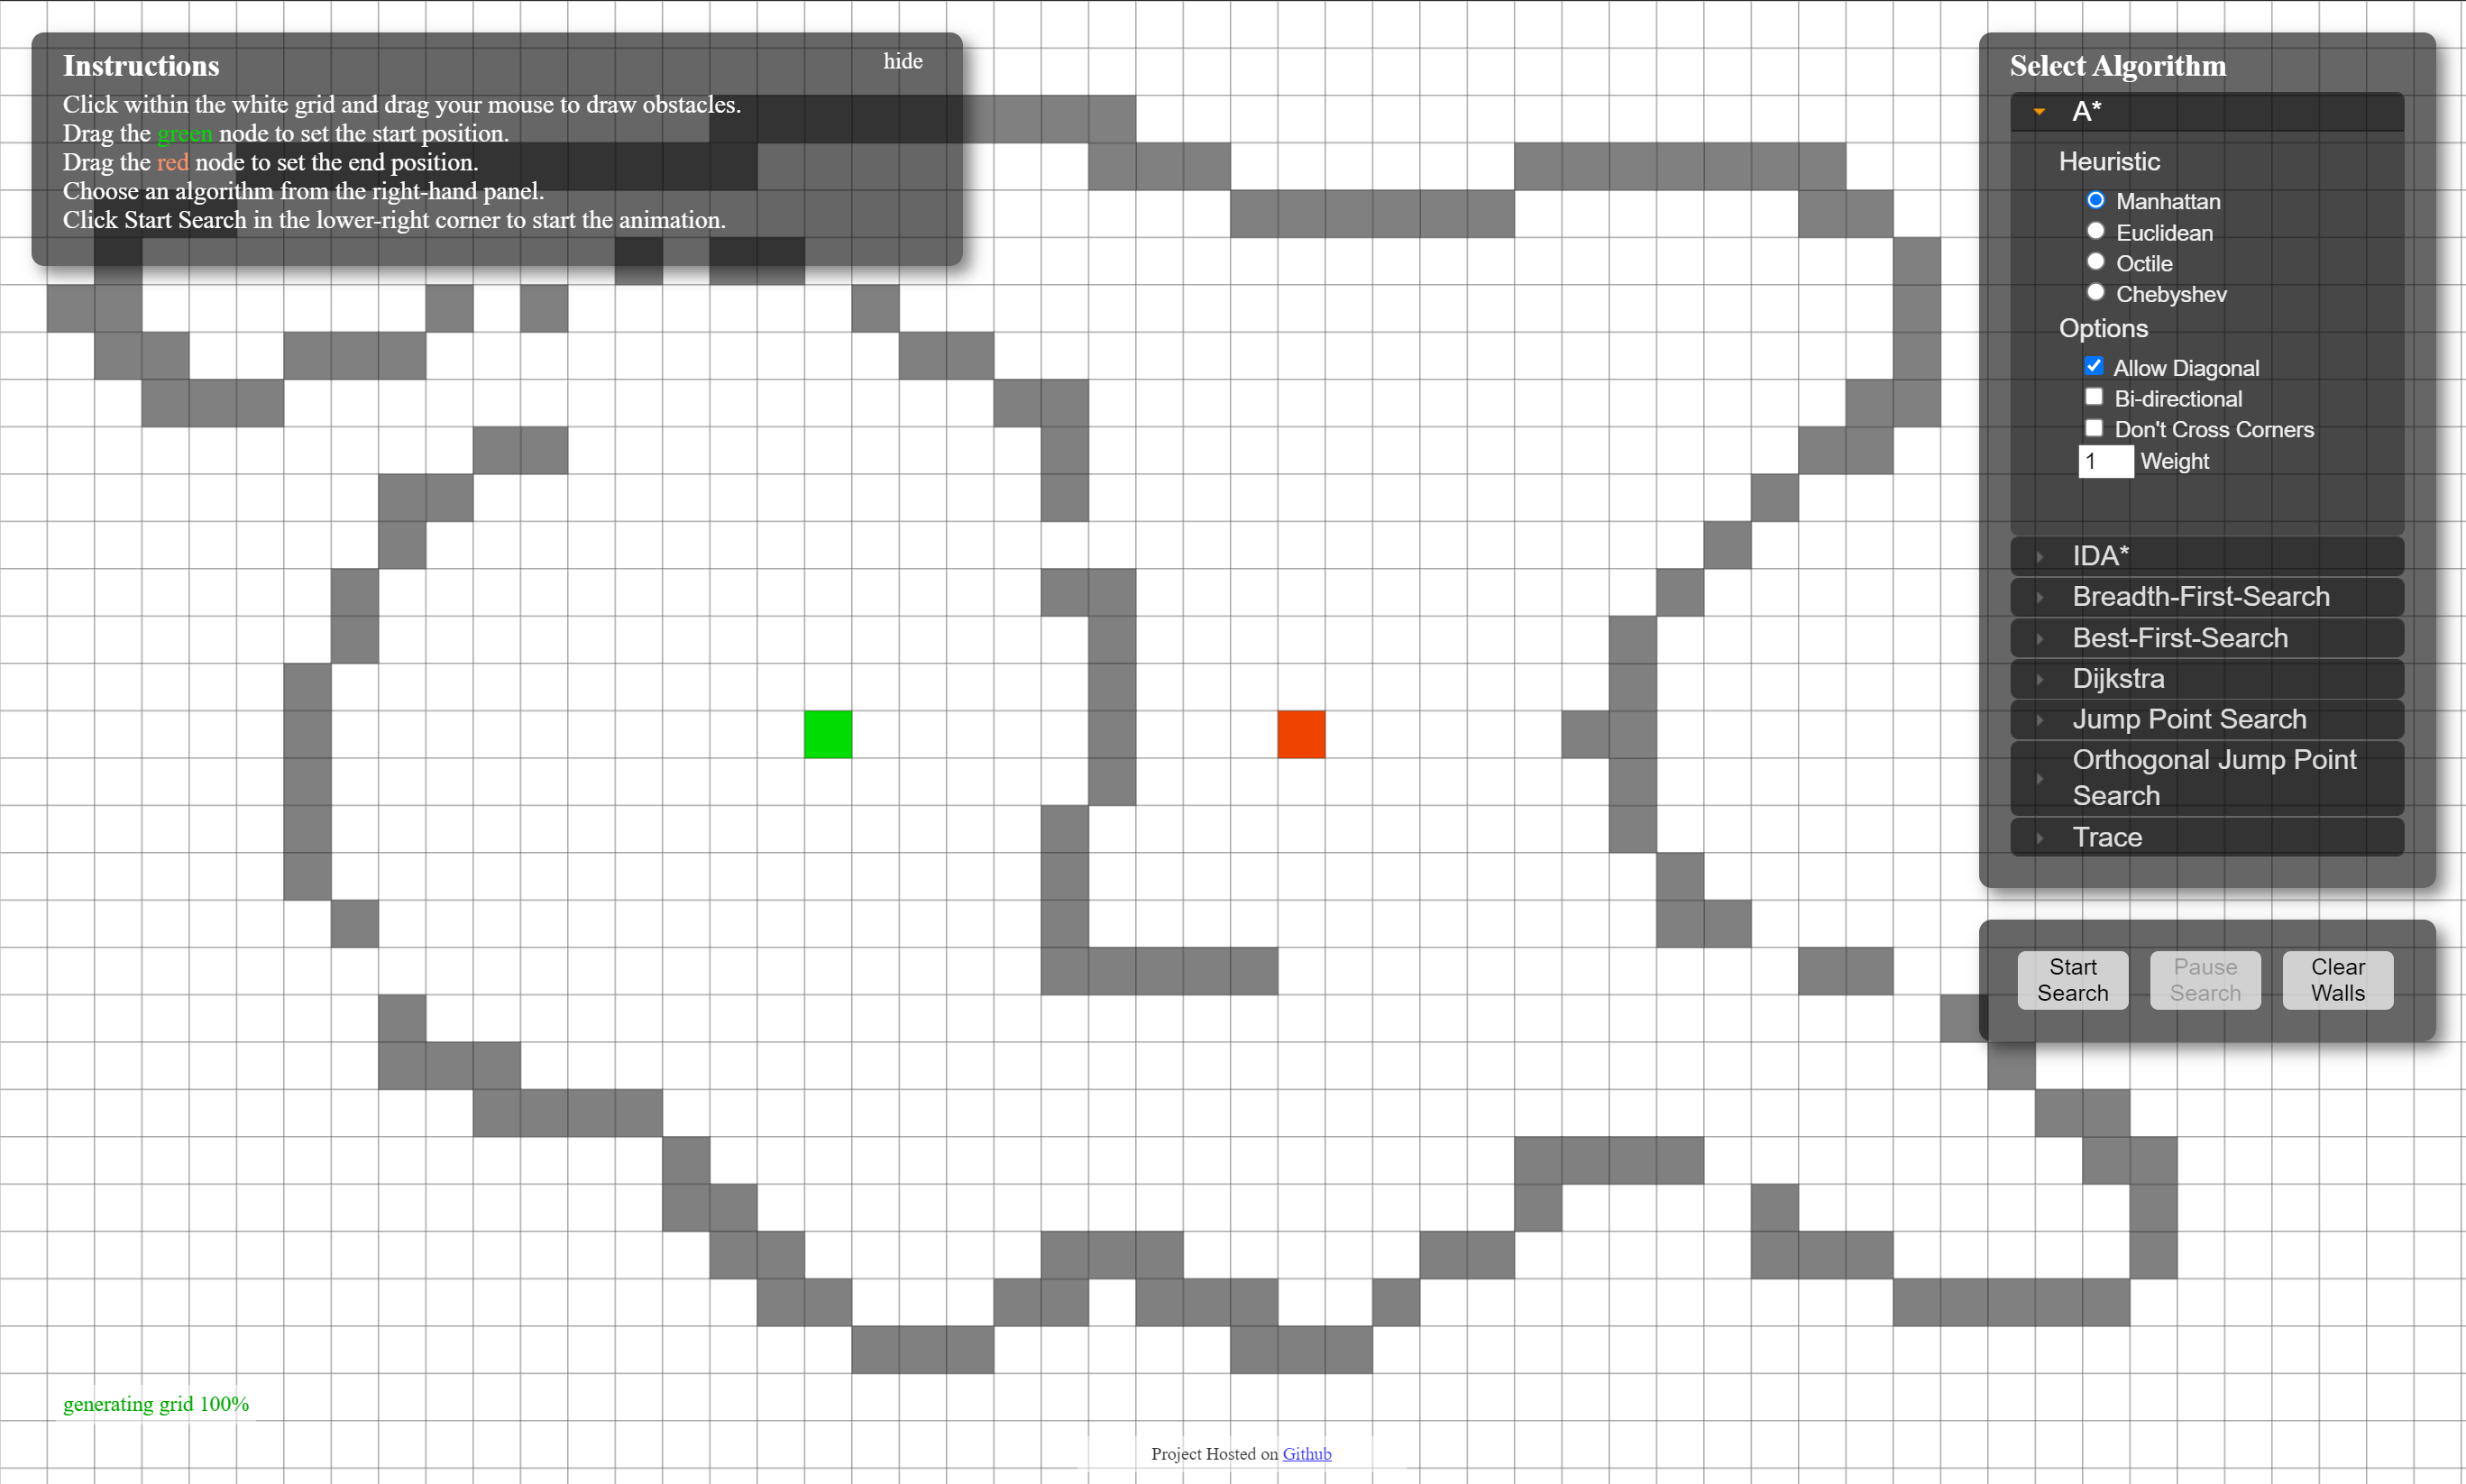
\includegraphics[width=\linewidth]{assets/Existing Solutions/example 2.PNG}
\subparagraph*{pros}
\begin{itemize}
    \item More options to choose from within each algorithm.
\end{itemize}
\subparagraph*{cons}
\begin{itemize}
    \item No maze generation.
    \item Visualization does not update when maze or start/finnish nodes are changed.
\end{itemize}


\paragraph{Example 3}
\href{https://pathfindout.com/
}{https://pathfindout.com/
}
\newline
In this example, mazes can be generated or drawn, however, mazes can only be generated with the recursive division algorithm. There are fewer path finding algorithms to solve the mazes than the others. The available algorithms are:
\begin{itemize}
    \item Dijkstra's Algorithm
    \item A* Search
    \item Breadth First Search
    \item Depth First Search
\end{itemize}
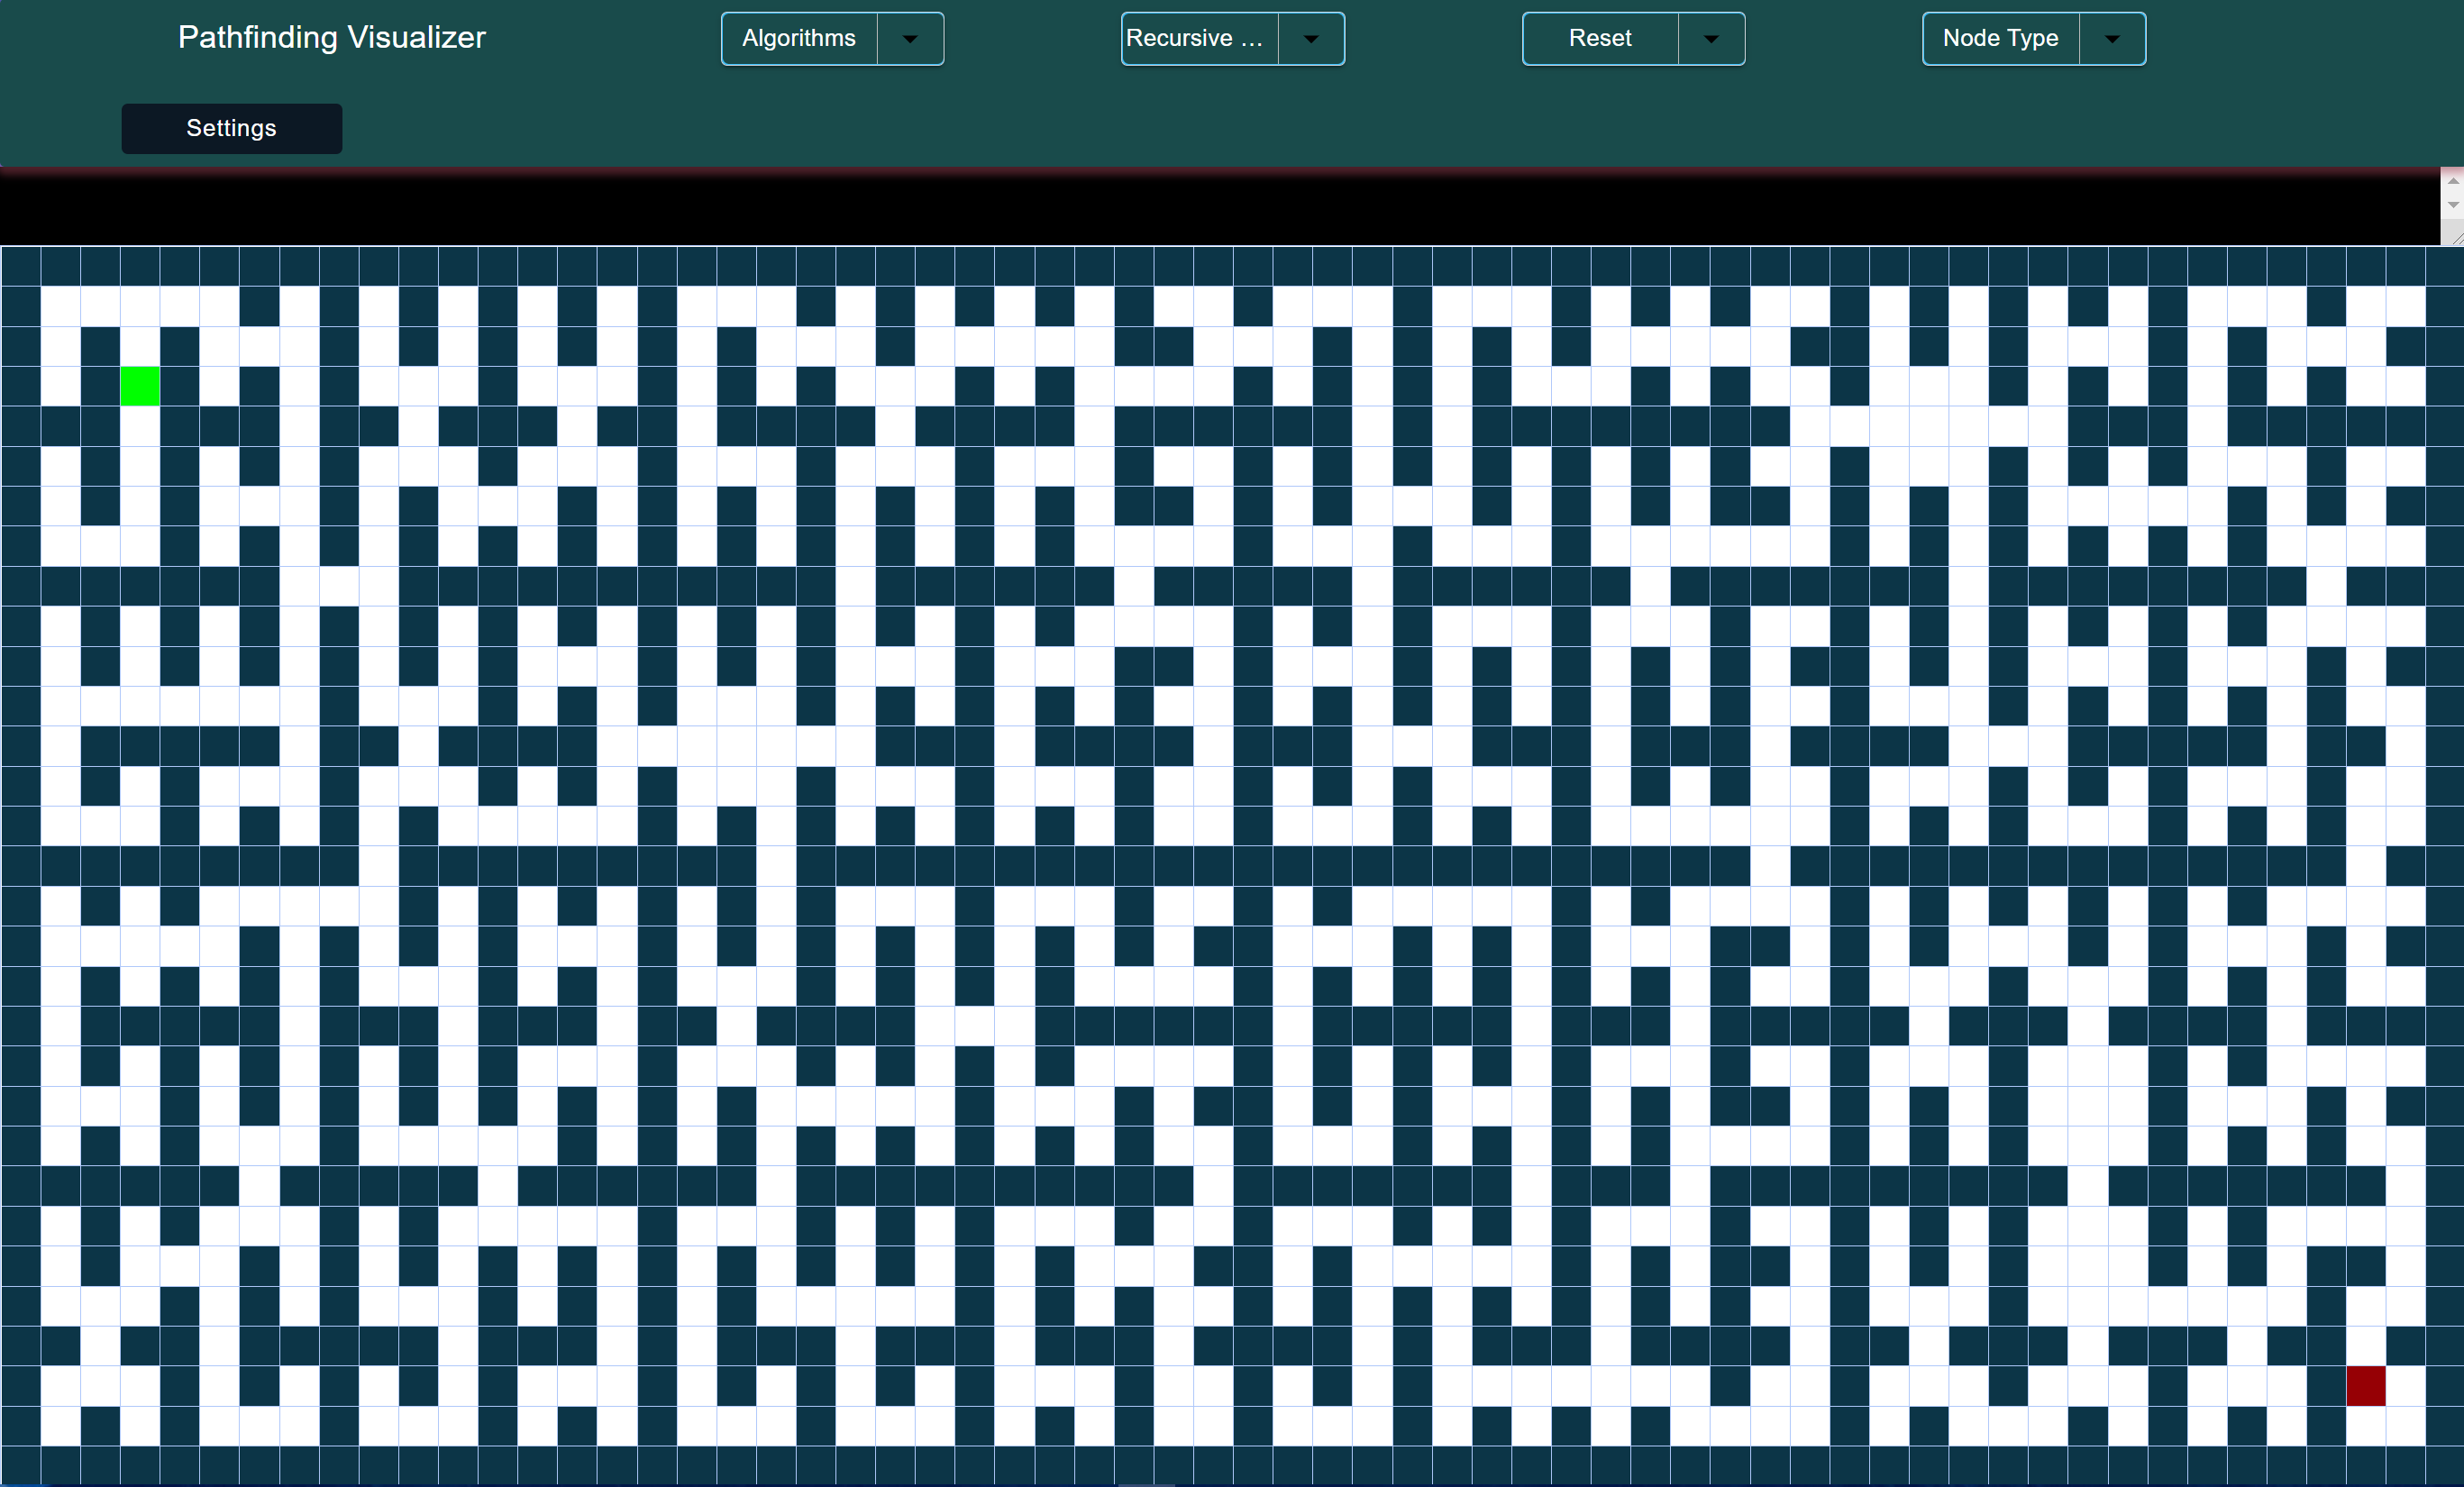
\includegraphics[width=\linewidth]{assets/Existing Solutions/example 3.PNG}
\subparagraph*{pros}
\begin{itemize}
    \item Different weighted nodes available.
    \item Shows how many nodes visited.
    \item Shows final path length.
    \item Data structure for some algorithms can be changed.
    \item Weights of specific node types can be changed.
    \item Node size can be changed.
\end{itemize}
\subparagraph*{cons}
\begin{itemize}
    \item Sometimes generates mazes that cannot be solved.
    \item Cannot edit maze after visualization has run.
    \item Only one maze generation algorithm.
    \item Fewer path finding algorithms to solve the maze.
\end{itemize}

\subsubsection{Proposed Solution}
I will make a path-finding visualization that encompasses as many of the merits of the existing solutions as possible, while also tackling as many of the drawbacks.
\begin{itemize}
    \item Research the different algorithms needed and write the corresponding pseudoscode.
    \item Create a mockup of the user interface.
    \item Create the user interface in react native.
    \item Code the algorithms in javascript.
    \item Add additional features suggested by end users.
    \item Test visualization and check that it meets all of the objectives.
\end{itemize}
\subsubsection{Prospective Users}
The users of this system will most likely consist of teachers and students who are learning about path finding algorithms as it will clearly show how the algorithms function.
\paragraph{Questions To Users}
I asked some prospective users some questions about what they would like to see in the visualizer.
\paragraph*{Questions}
\begin{enumerate}
    \item[Q1.]What algorithms would you like to see for maze generation?
    \item[Q2.]What algorithms would you like to see for solving the maze?
    \item[Q3.]What additional features would you like to see in the path finding visualization?
    \item[Q4.]Would it be useful to be able to write your own path finding algorithms that can be run in the visualization?  
\end{enumerate}
\paragraph*{Answers}
\begin{enumerate}
    \item[A1.]I would like to see recursive division and Prim's algorithms used for maze generation, as well as Kruskal's (less important). This is because Kruskal's and Prims are similar but each has their own advantages/disadvantages and recursive division is completely different.
    \item[A2.]I would like to see Dijkstra's algorithm and A* search, as these are very popular algorithms and one is a heuristic.
    \item[A3.]Option to add your own png image for the drawing of final path - "a sussy imposter running around the maze".
    \item[A4.]I would find it useful to be able to code my own algorithms. This would allow me to use the visualization with other, lesser known algorithms that I may need.
\end{enumerate}
The answers to these questions confirms what is required from the visualization, which will be reflected in the objectives. The need for contrasting algorithms is something that I will consider when deciding what algorithms to use.
\subsection{Objectives}
\subsubsection{Generate Mazes}
The website should be able to generate mazes using a number of different algorithms, including, but not limited to: Prim's algorithm, recursive division and random generation. There should also be a brief description of the algorithm that has been selected.

\subsubsection{User Drawn Mazes}
The user should be able to draw mazes and obstacles easily on the grid using the mouse.

\subsubsection{Solve Mazes}
The website should be able to solve mazes using a number of different algorithms, including, but not limited to: A* search, Dijkstra's algorithms, depth-first search and breadth-first search. There should also be a brief description of the algorithm that has been selected.

The website should also be able to take in an algorithm written by the user, and use it to solve the maze. This will be done by supplying documentation on what parameters need to be taken in and what will need to be returned from the function for the visualizer to work.
\subsubsection{Update Visualization}
If the maze is altered or and nodes moved once the visualization has been run, then it should update without rerunning the visualization

\subsubsection{Special Nodes}
There should be "special" nodes that are different from walls or space. For example, nodes with different weights or a "via point" node that the path must go through.
\section{Documented Design}
\subsection{Flow Chart}
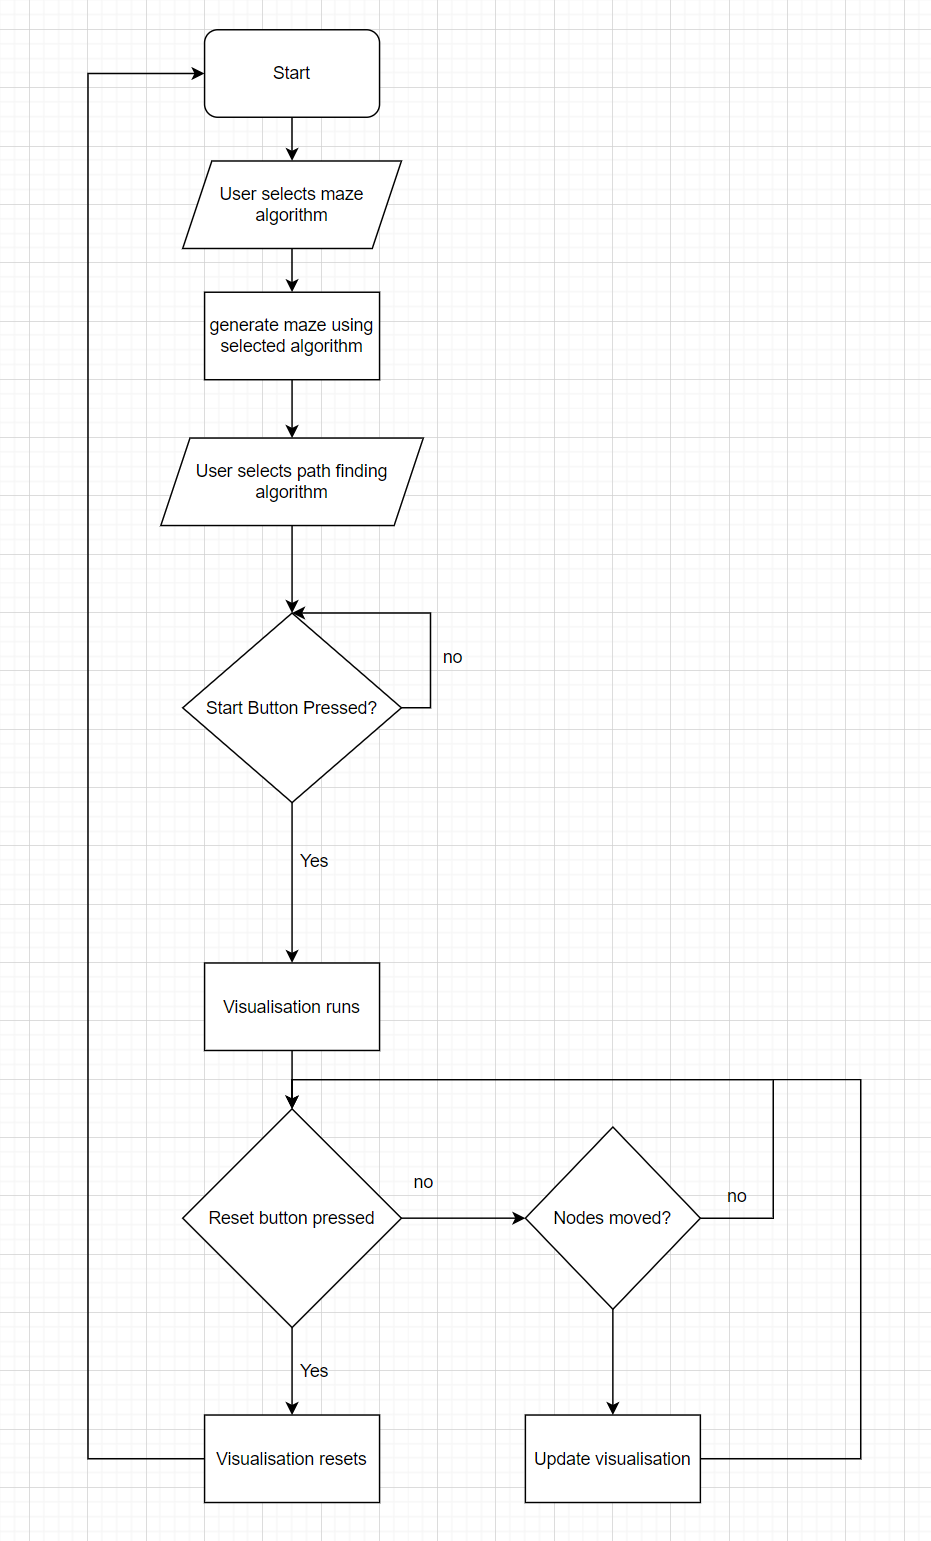
\includegraphics[width=\linewidth, height=17.5cm]{assets/flow chart.PNG}

\comment{
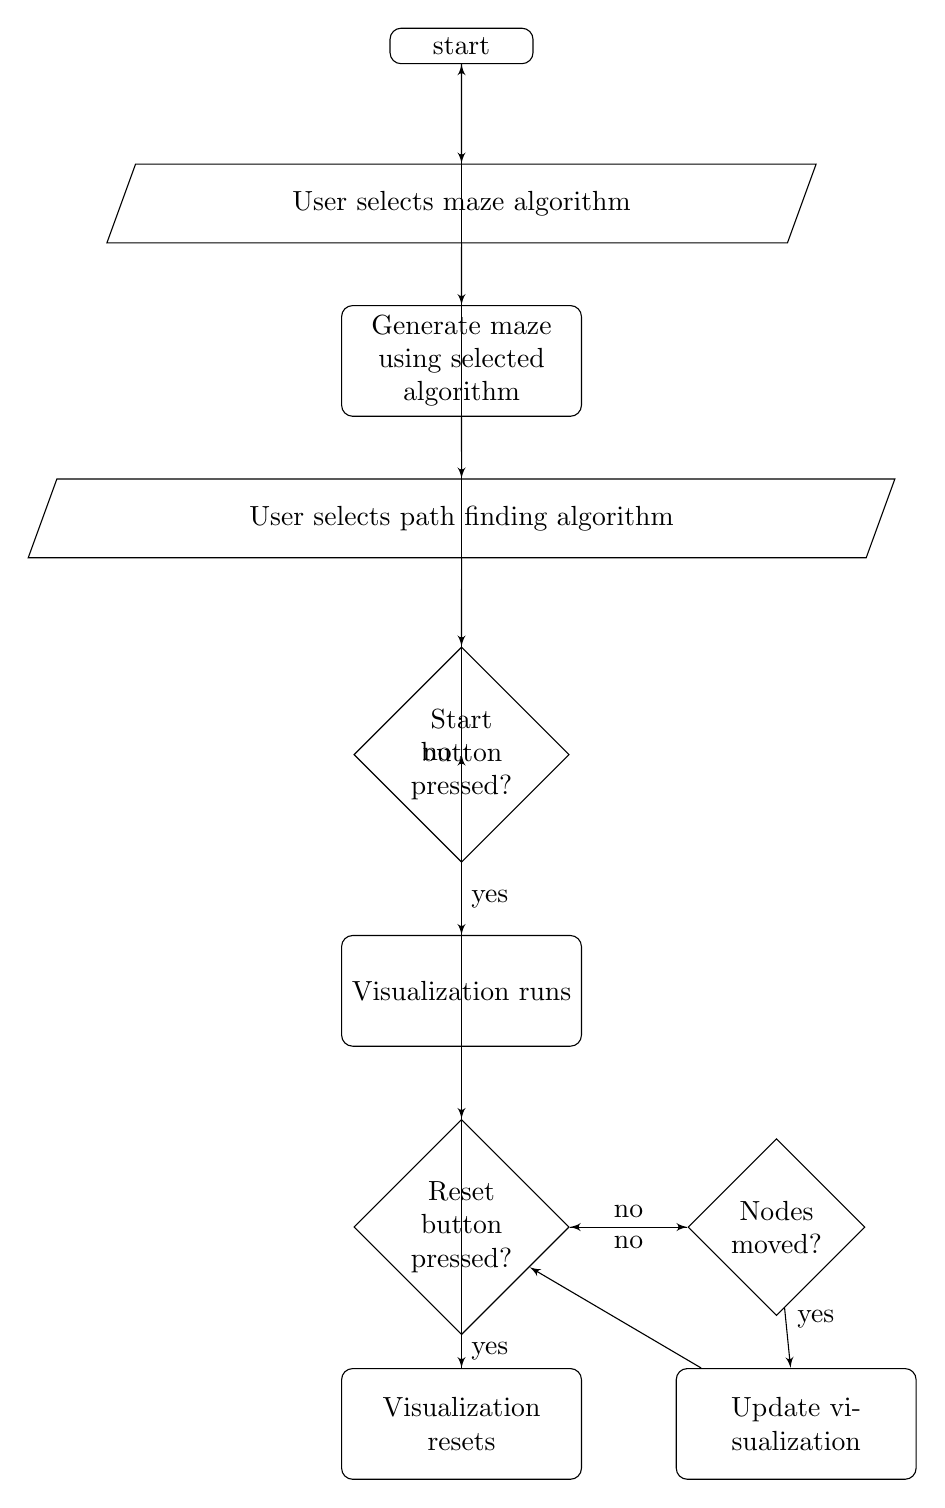
\begin{tikzpicture}[node distance = 2cm, auto]
    \node[start] (init) {start};
    \node [io, below of = init] (1) {User selects maze algorithm};
    \node[block, below of = 1] (2) {Generate maze using selected algorithm};
    \node [io, below of=2](3){User selects path finding algorithm};
    \node[decision, below of=3](4){Start button pressed?};
    \node[block, below of=4, yshift=-1cm](5){Visualization runs};
    \node[decision, below of=5](6){Reset button pressed?};
    \node[decision, right of=6, xshift=1cm](7){Nodes moved?};
    \node[block, below of=7, xshift=0.25cm, yshift=-0.5cm](8){Update visualization};
    \node[block, below of=6, yshift=-0.5cm](9){Visualization resets};

    \path[line] (init) -- (1);
    \path[line] (1) -- (2);
    \path[line] (2) -- (3);
    \path[line] (3) -- (4);
    \path[line] (4) -- node {no}(4);
    \path[line] (4) -- node {yes}(5);
    \path[line] (5) -- (6);
    \path[line] (6) -- node {no}(7);
    \path[line] (6) -- node {yes}(9);
    \path[line] (7) -- node {yes}(8);
    \path[line] (7) -- node {no}(6);
    \path[line] (8) -- (6);
    \path[line, anchor=west] (9) -- (init);
\end{tikzpicture}}

\subsection{User Interface}
I have used Figma to create a design mockup of how the user interface will look. This allows me to plan what user inputs will be needed.
\newline
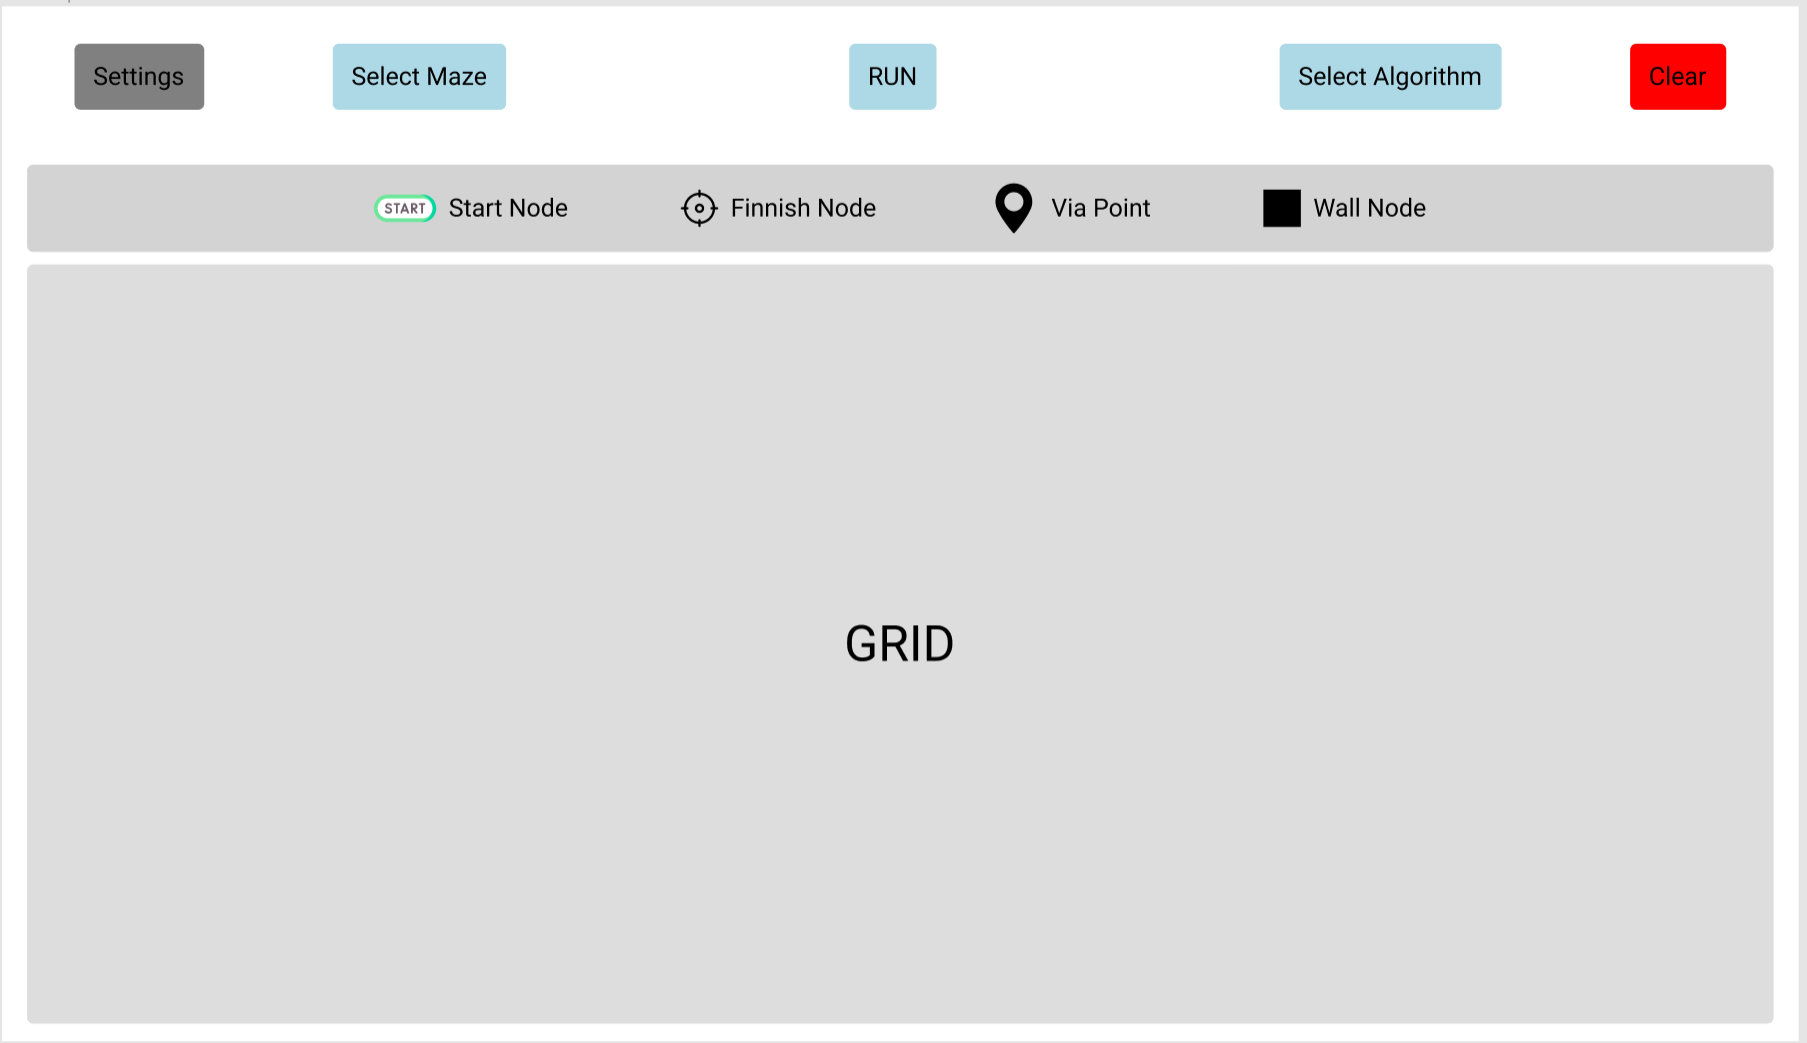
\includegraphics[width=\linewidth]{assets/gui.PNG}
\subsection{Class Diagrams}
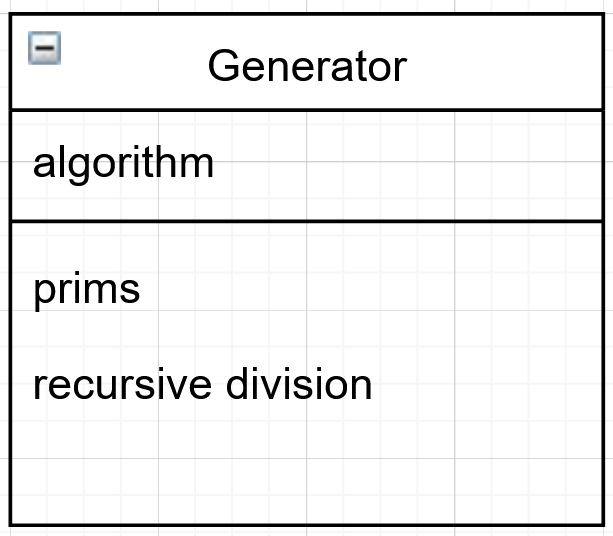
\includegraphics[width=0.5\linewidth]{assets/class diagrams/generator.PNG}
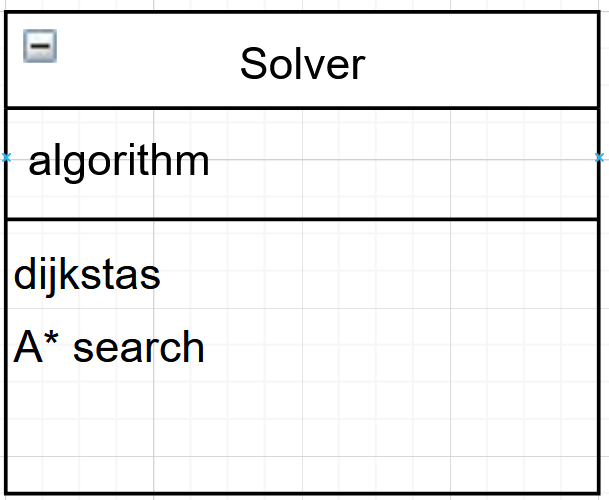
\includegraphics[width=0.5\linewidth]{assets/class diagrams/solver.PNG}
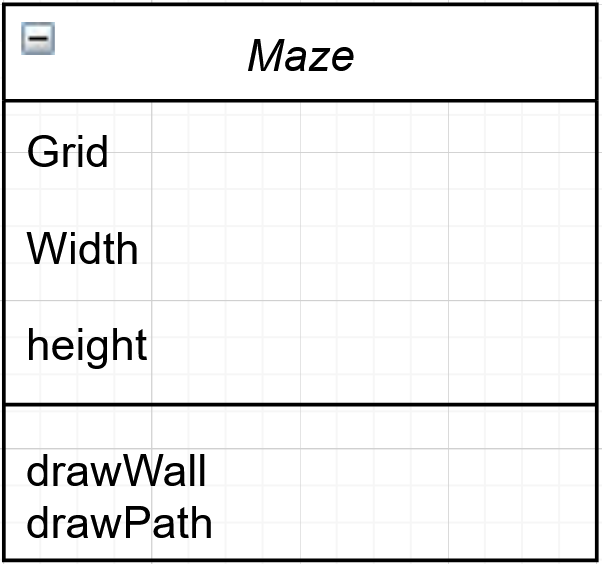
\includegraphics[width=0.5\linewidth]{assets/class diagrams/maze.PNG}
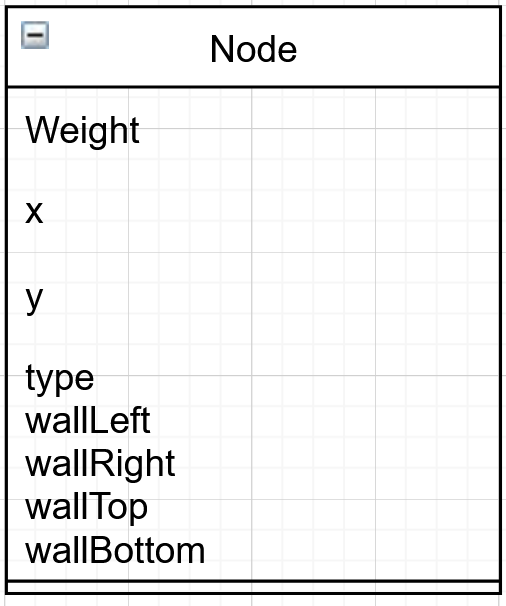
\includegraphics[width=0.5\linewidth]{assets/class diagrams/node.PNG}


\subsection{Data Strucure}
The Grid for the maze will be stored in a 2D array with each item being a Node with the information about it. For example, a 2x2 grid would look like: [[Node, Node], [Node, Node]]

\subsection{Algorithms}
\subsubsection{Maze generating algorithms}
\paragraph{prims}
\begin{verbatim}

    function prims(Grid){
        let start = [0,0]
        let inMaze = [start]
        let frontier = [
            [[start[0],start[1]+1],["left"]],
            [[start[0]+1, start[1]],["top"]]
        ]
        
        while (frontier.length > 0){
            let new = frontier.pop(randint(0, frontier.length - 1))
            let toAdd = new[0]
            let wall = new[1][randint(0, new[1].length - 1)]
            inMaze.push(toAdd)
            
            if (wall == "bottom"){
                Grid.grid[toAdd[0]][toAdd[1]].wallBottom = False
            }
            
            if (wall == "left"){
                Grid.grid[toAdd[0]][toAdd[1]].wallLeft = False
            }
            
            if (wall == "top" and toAdd[0] > 0){
                Grid.grid[toAdd[0]-1][toAdd[1]].wallBottom = False
            }
            
            if (wall == "right" and toAdd[1] < Grid.width){
                Grid.grid[toAdd[0]][toAdd[1]+1].wallLeft = False
            }
            
            let possible = [
                [toAdd[0]-1, toAdd[1]],
                [toAdd[0]+1,toAdd[1]],
                [toAdd[0],toAdd[1]-1],
                [toAdd[0], toAdd[1]+1]
            ]
            
            for i in range 4{
                p = possible[i]
                walls = ["bottom", "top", "right", "left"]
                wall = walls[i]
                
                if (0<=p[0]<Grid.height and 0<=p[1]<Grid.width){
                    if p not in inMaze{
                        found = False
                        for v in frontier{
                            if (v[0] == p){
                                v[1].push(wall)
                                found = True
                            }
                        }
                        if not found{
                            frontier.push([p, [wall]])
                        }
                    }
                }
            }
        }
    }
\end{verbatim}

\section{Evidence of Completeness}  
%out of 15 marks, argument for why the project is complete. Which algorithms have been used?

\section{Technical Solution}

\section{Testing}

\section{Evaluation}
\end{document}